\section{Equilibrium Analysis}

As Figure \ref{fig:Motion5} shows the leaf appears to settle to an equilibrium as it falls. To calculate the values of an equilibrium the time derivatives of equations \ref{eq:motion_eqns} %equation ref
can be set to zero so $\dot{u} = \dot{v} = \dot{\omega} = \dot{\theta} = 0$. These equations can be solved to find an equilibrium with $u=0, \theta=\frac{\pi}{2},\omega=0,v=\frac{-g}{k_{\parallel}}$. To calculate the stability of this equilibrium it is necessary to calculate the Jacobian of the system. The Jacobian will linearise the system around the equilibrium, the format of the Jacobian matrix is given in equation \ref{eq:Jacobian_eqn}.

\begin{equation}\label{eq:Jacobian_eqn}
\begin{bmatrix}
\frac{d\dot{u}}{du}&\frac{d\dot{u}}{dv}&\frac{d\dot{u}}{d\omega}&\frac{d\dot{u}}{d\theta}\\
\frac{d\dot{v}}{du}&\frac{d\dot{v}}{dv}&\frac{d\dot{v}}{d\omega}&\frac{d\dot{v}}{d\theta}\\
\frac{d\dot{\omega}}{du}&\frac{d\dot{\omega}}{dv}&\frac{d\dot{\omega}}{d\omega}&\frac{d\dot{\omega}}{d\theta}\\
\frac{d\dot{\theta}}{du}&\frac{d\dot{\theta}}{dv}&\frac{d\dot{\theta}}{d\omega}&\frac{d\dot{\theta}}{d\theta}
\end{bmatrix}
\end{equation}


% Is there a second equilibrium? Robert's v=v0-gt?

% Jacobian is too big for the page should we use the Jacobian evaluated at the equilibrium?
To investigate the stability of an equilibrium the Jacobian must be evaluated with the equilibrium values and the eigenvalues calculated. The Jacobian evaluated at the equilibrium is shown in equation \ref{eq:eval_Jacobian}.

\begin{equation}\label{eq:eval_Jacobian}
\begin{bmatrix}
 \frac{\pi g \rho}{k_{\parallel}}-k_{\perp}&0&0&-\frac{g\cdot(k_{\parallel}-k_{\perp})}{k_{\parallel}}-\frac{\pi g^2 \rho}{k_{\parallel}^2}\\
0&-k_{\parallel}&0&0\\
 \frac{-(3 \pi g \rho)}{l k_{\parallel}}&0&-k_{\perp}&\frac{3 \pi g^2 \rho}{l k_{\parallel}^2}\\
0&0&1&0
\end{bmatrix}
\end{equation}

This allows the eigenvalues to be calculated to determine the stability of the equilibrium. If the eigenvalues are negative the equilibrium is stable, if the eigenvalues are positive the equilibrium is unstable and if the eigenvalues are both positive and negative the equilibrium is a saddle. The system can have a local bifurcation at a parameter value if an eigenvalue passes through the imaginary axis. 

In Figure \ref{fig:Kper_Eig} the eigenvalues at the equilibrium are plotted for values of perpendicular friction between one and fifty. All other variables remained constant with $f=100, l=1, \rho = 0.1, g = 9.81$. There are both positive and negative real parts of the eigenvalues suggesting that the equilibrium is a saddle for these parameter values. It appears in Figure \ref{fig:Kper_Eig} as if some eigenvalues have zero real part. However, as Figure \ref{fig:Kper_Eig2} shows, the eigenvalues come close to zero but never reach it. 

\begin{figure}[H]
\centering
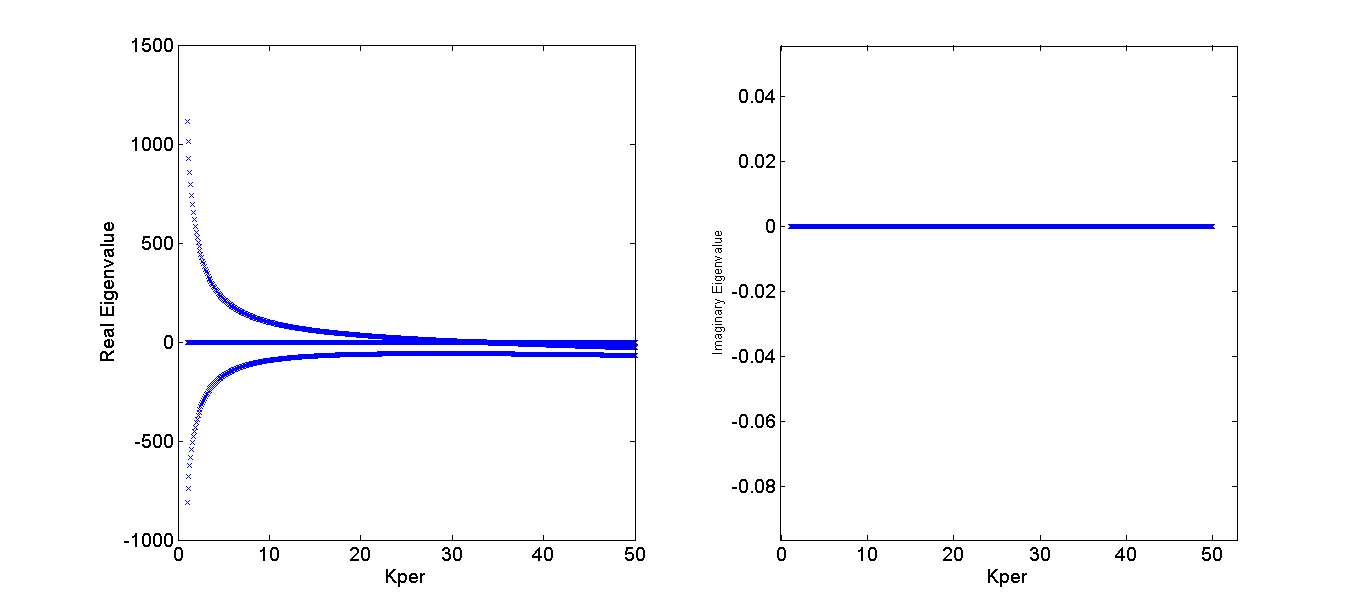
\includegraphics[width=0.7\textwidth]{Kper_Eigenvalues.png}
\caption{\label{fig:Kper_Eig}(Left)Plot showing the real part of the eigenvalues as the perpendicular friction is varied. (Right) Plot showing the imaginary part of the eigenvalues as the perpendicular friction is varied.
}
\end{figure}

\begin{figure}[H]
\centering
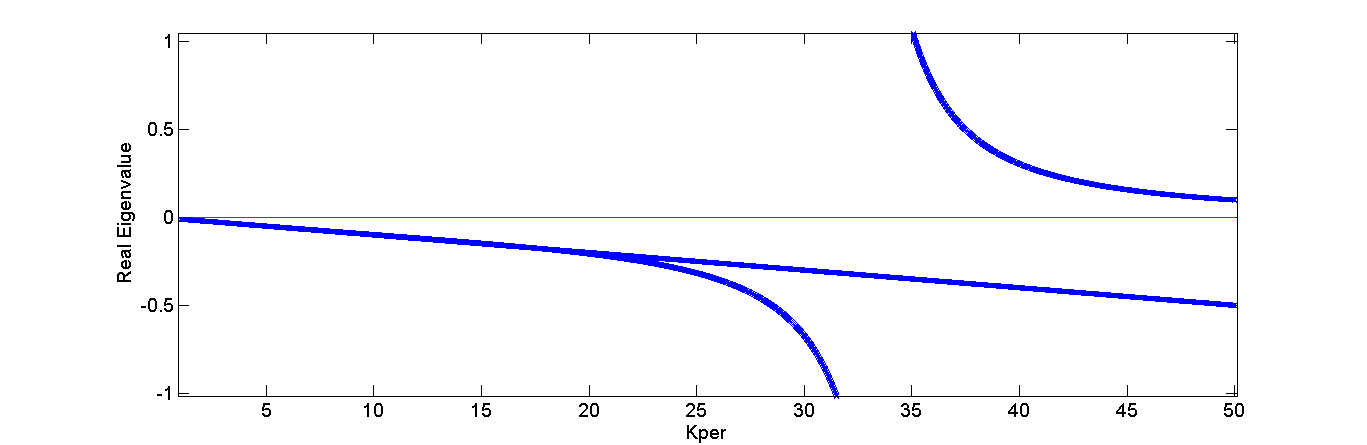
\includegraphics[width=0.7\textwidth]{Kper_Eigenvalues2.png}
\caption{\label{fig:Kper_Eig2}Plot showing the real part of the eigenvalues coming close to zero.
}
\end{figure}


This can be repeated for the remaining parameters f, l and $\rho$. 
The value of the perpendicular friction is fixed at 4.84 and $\rho$ is varied between 0.01 and 1. As $\rho$ is the ratio of the density of the fluid to that of the paper it is assumed it never equals zero. The eigenvalues are shown in Figure \ref{fig:Rho_Eig}. 

\begin{figure}[H]
\centering
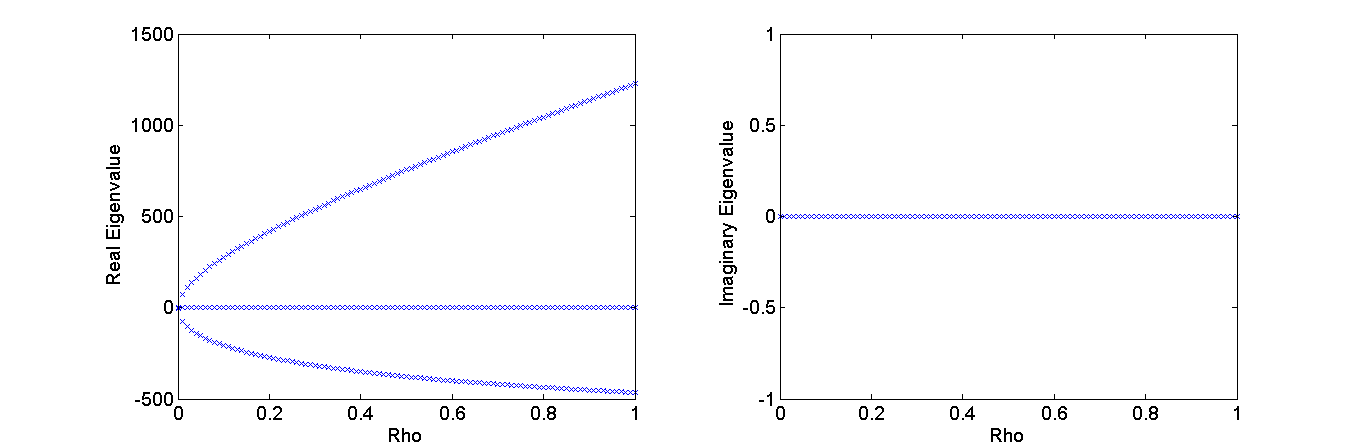
\includegraphics[width=0.7\textwidth]{Rho_Eigenvalues.png}
\caption{\label{fig:Rho_Eig}(Left)Plot showing the real part of the eigenvalues as $\rho$ is varied. (Right) Plot showing the imaginary part of the eigenvalues as $\rho$ is varied.
}
\end{figure}
As with the perpendicular fiction it appears as if the eigenvalues take a value of zero. However there are two eigenvalues with constant values, one at -0.04 and another at -0.0398. Again it can be seen there are eigenvalues with both positive and negative parts for all values of $\rho$ suggesting the equilibrium is a saddle for these parameter values. 

The value of $\rho$ is returned to 0.1 and the length of the leaf is investigated. The parameter l is varied between 0.01 and 2, it is assumed the leaf will not have zero length. Figure \ref{fig:l_Eig} shows the eigenvalues of the Jacobian for the range of l values.

\begin{figure}[H]
\centering
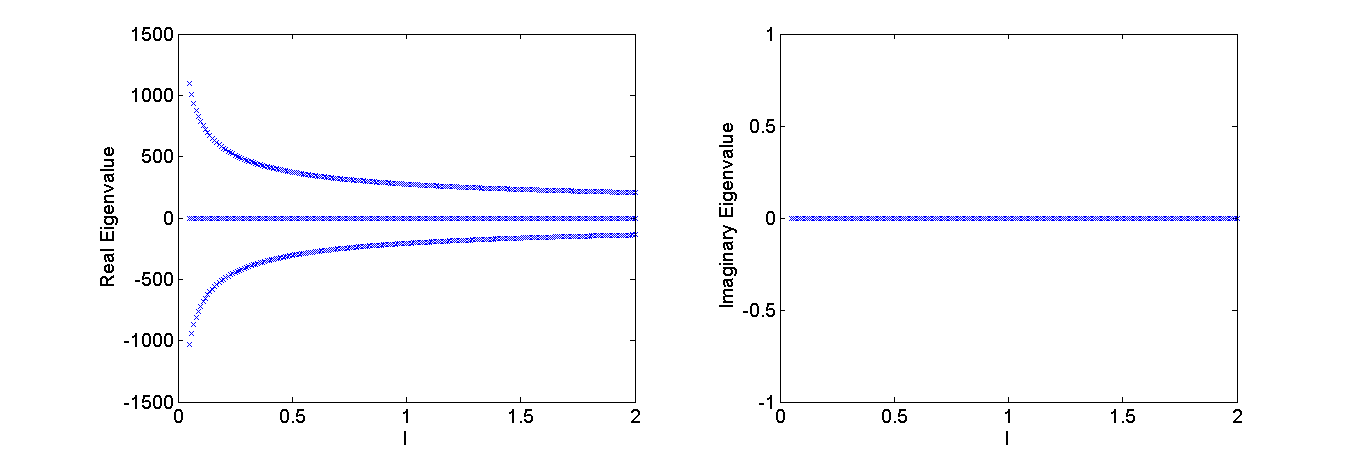
\includegraphics[width=0.7\textwidth]{l_Eigenvalues.png}
\caption{\label{fig:l_Eig}(Left)Plot showing the real part of the eigenvalues as the length is varied. (Right) Plot showing the imaginary part of the eigenvalues as the length is varied.
}
\end{figure}

As Figure \ref{fig:l_Eig} shows there are both positive and negative eigenvalues for all values of the parameter l which indicates the equilibrium is a saddle for this range of l values. As before there are no eigenvalues equal to zero, although some fall close but remain constant at -0.04.

The process is then repeated, setting l to 1 and varying f in the range $0.1<f<150$. The eigenvalues are shown in Figure \ref{fig:f_Eig}. 

\begin{figure}[H]
\centering
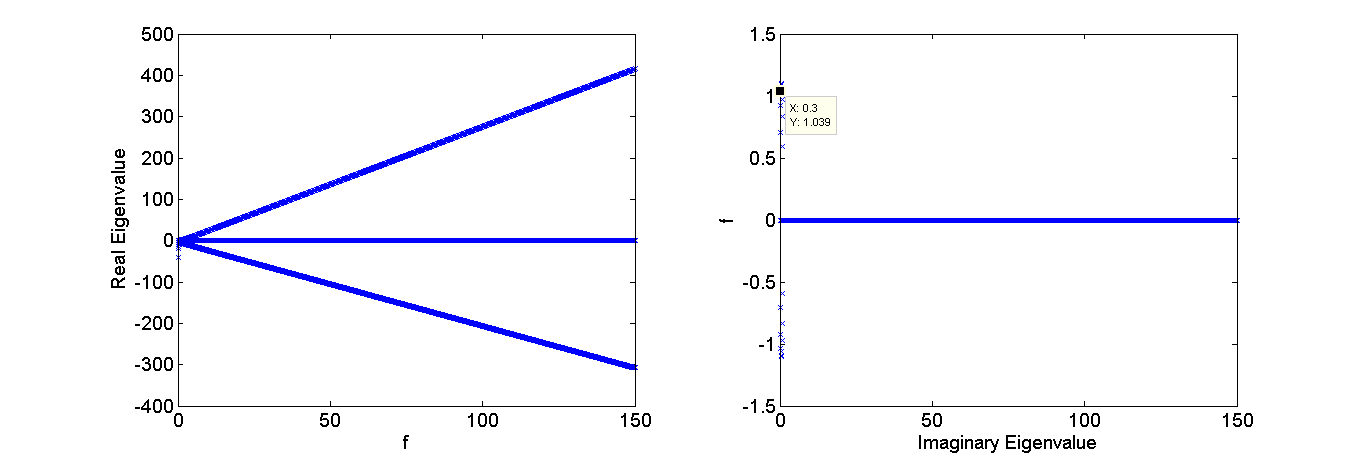
\includegraphics[width=0.7\textwidth]{f_Eigenvalues.png}
\caption{\label{fig:f_Eig}(Left)Plot showing the real part of the eigenvalues as f is varied. (Right) Plot showing the imaginary part of the eigenvalues as f is varied.
}
\end{figure}
As Figure \ref{fig:f_Eig} shows as f increases two eigenvalues increase while two remain constant near zero. For smaller values of f, two of the eigenvalues have a complex part. This is shown in Figure \ref{fig:f_Eig2}.

\begin{figure}[H]
\centering
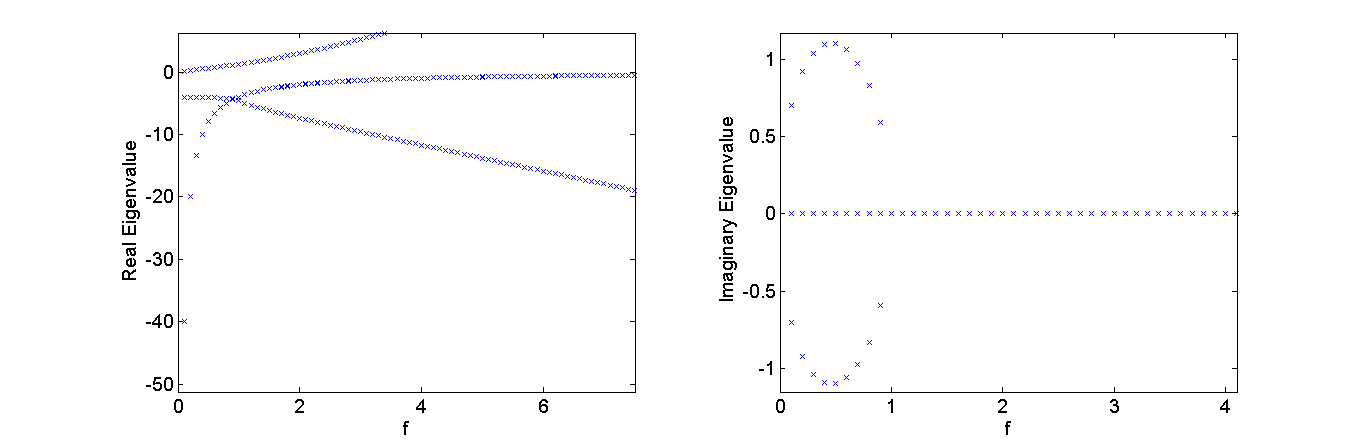
\includegraphics[width=0.7\textwidth]{f_Eigenvalues2.png}
\caption{\label{fig:f_Eig2}(Left)Plot showing the real part of the eigenvalues as f is varied. (Right) Plot showing the imaginary part of the eigenvalues as f is varied.
}
\end{figure}
For values of f less than one some eigenvalues have an imaginary part. % What does this tell us?
Again there are both positive and negative eigenvalues which indicates the equilibrium is a saddle for all values of f in the range. There are no eigenvalues with zero real part, so no bifurcations occur for these parameter values. 


% Evaluate Jacobian at equilibrium, plot graphs of eigenvalues change parameters and comment on changes in stability. Look for bifurcations.  


